\documentclass[a4paper]{article}

%%%%%%%% CREATE DOCUMENT STRUCTURE %%%%%%%%
%% Language and font encodings
\usepackage[english]{babel}
\usepackage[utf8x]{inputenc}
\usepackage[T1]{fontenc}
\usepackage{lmodern,textcomp}
%\usepackage{subfig}

\usepackage{pdflscape}

%% Sets page size and margins
\usepackage[a4paper,top=3cm,bottom=2cm,left=2cm,right=2cm,marginparwidth=1.75cm]{geometry}

%% Useful packages
\usepackage{amsmath}
\usepackage{graphicx}
\usepackage[colorinlistoftodos]{todonotes}
\usepackage[colorlinks=true, allcolors=blue]{hyperref}
\usepackage{caption}
\usepackage{subcaption}
\usepackage{sectsty}
\usepackage{apacite}
\usepackage{float}
\usepackage{titling} 
\usepackage{blindtext}
\usepackage[square,sort,comma,numbers]{natbib}
\usepackage[colorinlistoftodos]{todonotes}
\usepackage{xcolor}
\definecolor{darkgreen}{rgb}{0.0, 0.4, 0.0}

\usepackage{lipsum}

%% Gantt chart package
\usepackage{pgfgantt}

%% Start sections on new pages
\usepackage{titlesec}
\newcommand{\sectionbreak}{\clearpage}

%% Wrap figures
\usepackage{wrapfig}

%%%%%%%% DOCUMENT %%%%%%%%
\begin{document}

%%%% Title Page
\begin{titlepage}

\newcommand{\HRule}{\rule{\linewidth}{0.5mm}} 							% horizontal line and its thickness
\center 
 
% University
\textsc{\LARGE The Hague University of Applied Sciences}\\[1cm]

% Document info
\textsc{\Large Advanced real-time systems}\\[0.2cm]
\textsc{\large lab}\\[1cm] 										% Course Code
\HRule \\[0.8cm]
{ \huge \bfseries Final Report}\\[0.7cm]								% Assignment
\HRule \\[2cm]
\large
\emph{Author/Student:}\\
Luca van Straaten (18073611)\\[1.5cm]													% Author info
\emph{Instructor:}\\
X. van Rijnsoever\\[1.5cm]										
{\large \today}\\[5cm]

\includegraphics[width=0.6\textwidth]{images/hhs.png}\\[1cm] 	% University logo
\vfill
%update the version of document each time its modified after review
Document version 1.0
\end{titlepage}


\newpage
  \pagenumbering{roman}
  \tableofcontents
\newpage
\pagenumbering{arabic}

%%\begin{abstract}
%%Your abstract.
%%\end{abstract}

%%%% SECTIONS
\input{content/Introduction}
\section {Assignment 1 \\ {Setup}}
\label {sec:assignment_1}

For this assignment we connected the Camera to the Virtual Machine. And to the project tempalte a case was addet to the "switch (key)" statement. This case was used to take a picture with the camera. The picture was then saved in the folder from wich the program was run.

\begin{lstlisting}[language=C, caption=save image to file]
    case 's':
        cout << "Saving..." << endl;
        // save image using openCV API
        imwrite("blahai.png", image);
\end{lstlisting}

We pointed the camera at an object and adjusted the apature and focus to get a good looking picture with a shutter time of 100ms. See image \ref{img:blahai}

\section {Assignment 2 \\ {Object in front of Dark Background}}
\label {sec:assignment_2}


\section {Assignment 3 \\ {Moving Object}}
\label {sec:assignment_3}

Take an image of a considerably fast moving object (rotating disk) without any motion-blur and without reflection from any light-sources. You will not be able to synchronize the camera, so find a solution which will not need any synchronization.
Make a sketch of the required setup first, discuss multiple solutions in the group. \cite{Lab_Assignments}



\begin{lstlisting}[language=C, caption=save image to file, label=lst:50loop]
// capture 50 frames
if (capt50 == true) {
    capt50 = false;
    for(int i = 0; i < 50; i++) {
        cam0.captureFrame(&image);
        // save image with frame number
        imwrite("../capt/img" + to_string(i) + ".png", image);
    }
}
\end{lstlisting}


\subsection{Optimal exposure}

We use a strobe light to expose this image. The stroke frequency is not important but should be sufficiently slow to make it impossible for two exposures to occur in a single frame, and it should also be slow so that the capacitors inside the strobe enough time to charge to give the lights its maximum brightness. We took 50 images, and saved them to the file system. The first image which looks like \ref{fig:img36} was handpicked and the other images ware ignored.

\begin{figure}[h!]
    \centering
    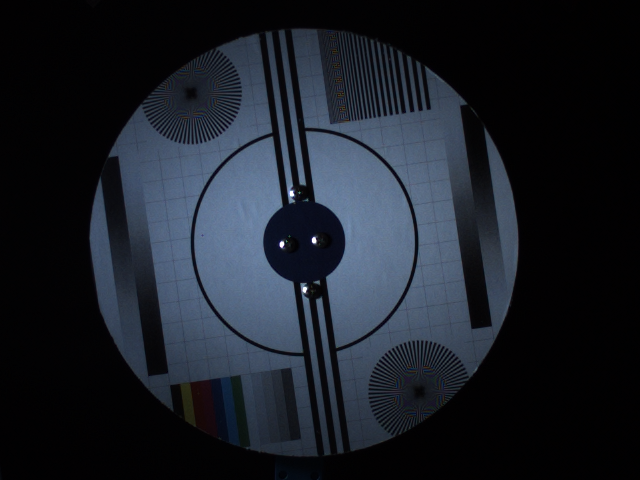
\includegraphics[width=0.35\textwidth]{img36.png}
    \caption{Image of moving object}
    \label{fig:img36}
\end{figure}

\subsection{Sketch of setup}

\begin{figure}[h!]
    \centering
    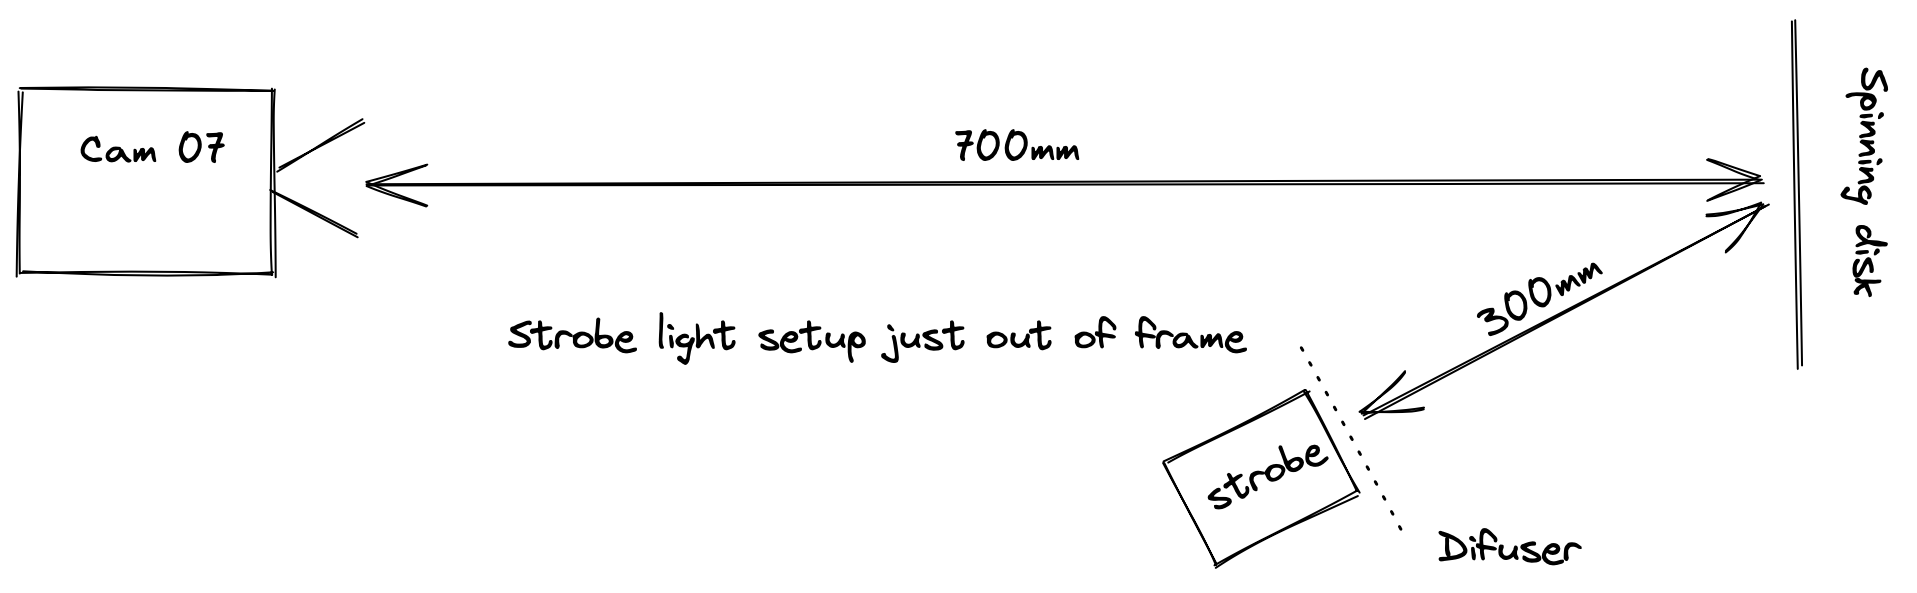
\includegraphics[width=0.65\textwidth]{Lab_3_Diagram.png}
    \caption{Sketch of setup}
    \label{fig:Lab_3_Diagram}
\end{figure}

\subsection{Calculation of ‘angle of view’}

We use the same camera and lens as assignment two, So the angle of view will be identical as calculated in section \ref{sec:angle_of_view}.
\section {Assignment 4 \\ {Salt and Pepper Noise}}
\label {sec:assignment_4}

\subsection{Manipulate own image from assignment 2}

We applyed a salt and pepper noise filter to the image from assignment 2. The image is shown in figure \ref{fig:fortGT_Noise}.

\begin{figure}[h!]
    \centering
    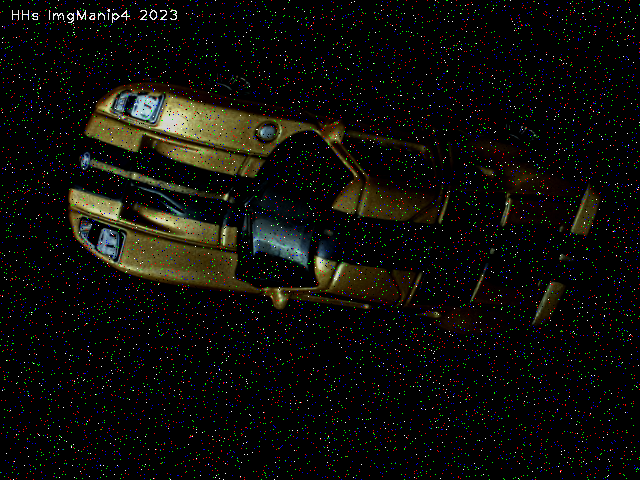
\includegraphics[width=0.45\textwidth]{fortGT_Noise.png}
    \caption{Image with salt and pepper noise}
    \label{fig:fortGT_Noise}
\end{figure}

\subsection{Write C/C++ code for Brightness correction}

\subsection{Write C/C++ code for ‘Salt and Pepper Noise’ correction}

A ‘Salt and Pepper Noise’ correction filter was written and can be found in appendix \ref{sec:appendix_B}. The filter function is shown in listing \ref{lst:noise_filter}.

\begin{lstlisting}[language=C, caption=Noise correction filter, label=lst:noise_filter]
    void filter(Mat input, Mat& result) {
        Size s = input.size();
        long h, w;
        long sum;
        
        std::cout << "Input type was : " << input.type() << std::endl;
        uint8_t out[s.height][s.width];
        
        std::cout << s.height << " " << s.width << std::endl;
        
        for (w=0; w<s.width; w++){
            for(h=0; h<s.height; h++){
                sum = 0;
                std::vector<uint8_t> median;
                
                for (int _x = -1; _x < 2; ++_x)
                {
                    for (int _y = -1; _y < 2; ++_y)
                    {
                        int idx_y = h + _y;
                        int idx_x = w + _x;
                        
                        if (idx_x < 0 || idx_x > s.width)
                            break;
                            
                        if (idx_y < 0 || idx_y > s.height)
                            break;
                        
                        median.push_back(input.at<uint8_t>(idx_y,idx_x));
                    }
                }
                std::sort(std::begin(median), std::end(median));
                        
                for (auto it = median.begin(); it != median.end(); ++it) {
                    sum = median.at(median.size()/2);
                }
                out[h][w]=(uint8_t)sum;
            }
        }
        result = Mat(s.height, s.width, CV_8U, out); //or maybe CV_8UC1?
        Size _s = result.size();
        std::cout << "done: " << _s.height << " " << _s.width << std::endl;
    }
    }
\end{lstlisting}

\section {Assignment 5 \\ {Convolution}}
\label {sec:assignment_5}


\section {Assignment 6 \\ {Demosaicing Filter}}
\label {sec:assignment_6}

\subsection{Write C/C++ code for capturing a raw image}

\begin{lstlisting}[language=C, caption=save image to file, label=lst:rawcode]
// capture raw image
imshow(camName, image);
if (captRAW == true) {
    captRAW = false;
    // save raw image
    cfg.camMode = CAM_MODE_RAW;
    cam0.captureFrame(&image);
    imwrite("../capt/RAW.png", image);

    // save color image
    cfg.camMode = CAM_MODE_COL;
    cam0.captureFrame(&image);
    imwrite("../capt/COL.png", image);
}
\end{lstlisting}

%%%%%%%% EXTRA TIPS %%%%%%%%
%% hou deze structuur aan voor afbeeldingen
%%\begin{figure}[H]
%%\includegraphics[]{Pendulum.jpg}
%%\caption{Sketch of the pendulum}
%%\label{fig:pendulum}
%%\end{figure}


\newpage
\bibliographystyle{apacite}
\bibliography{ref}

\end{document}